\documentclass[11pt]{article}
\usepackage{icmlko}
\begin{document}

\title{펀딩 $+0.42$ 는 세상이 아니라 우리가 뜬 400건의 성질이었다}
\author{월드모델 실험실}
\date{노트 379 · 2026년 8월 1일}
\maketitle

\begin{abstract}
노트 374가 텀블벅 목록이 인기순이고 우리 펀딩 400건이 상위 19\%라는 것을
쟀고, 노트 375가 그것을 \emph{구역 편향}이라 이름 붙였다. 값을 재려면
대표 표본이 필요해 씨앗 고정 균일 표본 \textbf{2,500건}을 모았다. 다
모였다.

\textbf{목록은 생각보다 더 심하게 정렬돼 있다} --- 균일 표본 안에서
쪽수와 라벨의 상관이 $-0.6944$ 이고(노트 374의 $-0.3666$ 은 좁은 옛
표본에서 잰 것이었다), 후원자 중앙이 옛 400건 \textbf{139명} 대 균일
2,500건 \textbf{37명}이다.

\textbf{그래서 값을 쟀다.} 균일 표본의 2025년 이후 449건을 \emph{유보에만}
넣고 학습 320행은 손대지 않은 채 한 번의 적합 안에서 갈랐다:

\begin{center}
옛 유보(위 19\%) 80행 $\mathbf{+0.3746}$ \quad 대 \quad
균일 유보 449행 $\mathbf{+0.1012}$
\end{center}

퍼짐 탓이 아니다 --- 새 쪽이 오히려 \emph{넓다}(0.621 대 0.407).
\textbf{옛 것과 같은 라벨 구간}으로 잘라도(292행, 퍼짐 0.422) $+0.0667$
이고, 옛 바닥 아래 157행은 $-0.0094$ 다. 균일 쪽에서 옛 퍼짐에 맞춘 연속
창 551개의 5\,--\,95\% 띠가 $[+0.0274,\ +0.1559]$ 인데 옛 것의 $+0.3746$
은 \textbf{100번째 백분위}, 개수를 맞춘 80행 무작위 대조에서도 99번째다.
그리고 예측이 죽은 것도 아니다 --- 449행에 서로 다른 예측이 434개다
(노트 377의 빈칸형과 다르다).

\textbf{채택했다.} 자료 결정이고 씨앗이 고정돼 재현되며, 옛 400행의 축과
라벨이 100\% 그대로이고 학습이 안 늘었다. 새 챔피언은 \textbf{판 0.4057 ·
분모 3,430} 이다.

\textbf{그런데 내려간 것의 86\%는 정직해진 몫이 아니다.} 판 $0.4620 \to
0.4057$ 중 펀딩 수치가 옳아진 몫은 $-0.0078$ 뿐이고 나머지 $-0.0486$ 은
펀딩의 \emph{무게}가 80에서 529로 6.6배가 된 몫이다. 무게가 유보 행 수라
\textbf{판은 도메인의 중요도가 아니라 우리의 수집 노력을 가중치로 쓰고
있다.} 다음 항목은 그것이다.
\end{abstract}

\section{쟀다}

\begin{figure}[t]
\centering
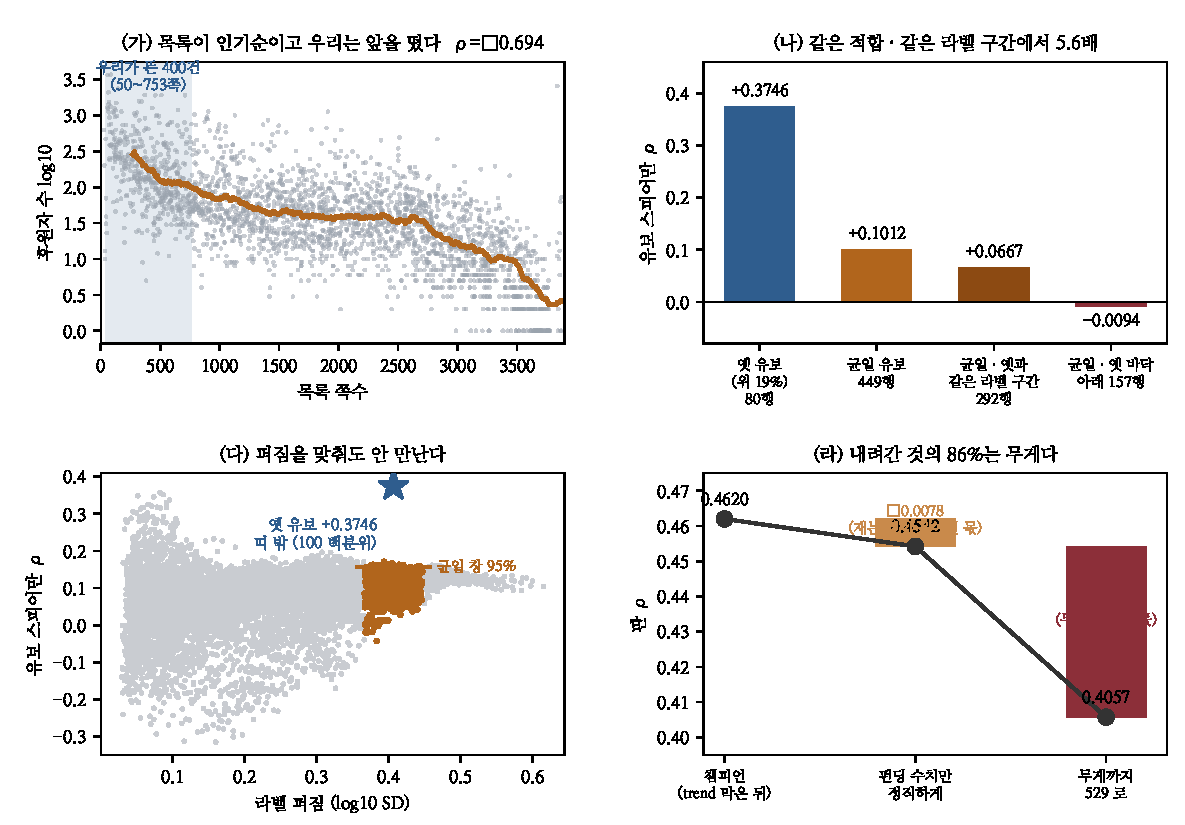
\includegraphics[width=\linewidth]{figs/fig379.pdf}
\caption{\textbf{(가)} 균일 2,500건의 쪽수 대 라벨. 주황은 120건 이동평균.
파란 띠가 우리가 뜬 구역(50\,--\,753쪽)이다. \textbf{(나)} 같은 적합
안에서 가른 넷. \textbf{(다)} 균일 쪽에서 옛 퍼짐(0.407)에 맞춘 연속 창
551개의 분포와 옛 유보의 위치 --- 띠 밖이다. \textbf{(라)} 판이 내려간
몫을 가르면 재는 것이 옳아진 몫은 $-0.0078$, 무게가 바뀐 몫이 $-0.0486$
이다.}
\label{fig:main}
\end{figure}

\textbf{절차는 노트 372 · 376과 같다.} 새 행은 유보에만 넣고 학습은
고정한 채 \emph{한 번의 적합 안에서} 가른다 --- 따로 적합시키면 도메인
칸의 부호가 열에 넷 뒤집힌다(노트 358).

축은 \texttt{ingest/funding\_axes.py} 를 그대로 돌려 만들었다. 창작자
사전 건수는 표본 안에서 세지 않고 전체 목록 색인을 쓰므로(그 함수의
주석이 이미 경고해 뒀다) 표본 크기가 축을 흔들지 않는다.

\textbf{위험 점검.} 옛 400행의 공유 축 다섯이 전부 100\% 그대로이고
($|$차$|$ 평균 0.0000), 라벨이 바뀐 행이 0이며, 새로 든 449건 중 학습으로
가는 행이 0이다.

\begin{center}
\begin{tabular}{lrrr}
\hline
무리 & 행 & 라벨 퍼짐 & $\rho$ \\
\hline
옛 유보 (위 19\%) & 80 & 0.407 & $+0.3746$ \\
균일 유보 & 449 & 0.621 & $+0.1012$ \\
\quad 그중 옛과 같은 라벨 구간 & 292 & 0.422 & $+0.0667$ \\
\quad 그중 옛 바닥 아래 & 157 & 0.359 & $-0.0094$ \\
전부 & 529 & 0.628 & $+0.0853$ \\
\hline
\end{tabular}
\end{center}

\section{퍼짐도 개수도 아니다}

노트 376이 좁은 퍼짐이 $\rho$ 를 깎는다는 것을 보였으니 여기서도 먼저
의심해야 한다. \textbf{그런데 방향이 반대다} --- 새 쪽 퍼짐이 0.621 로
옛 쪽 0.407 보다 \emph{넓다}. 넓은 범위는 보통 상관을 \emph{올린다}.

그래도 갈랐다. 셋 다 같은 쪽을 가리킨다.

\textbf{첫째, 같은 라벨 구간.} 옛 유보의 구간($1.230 \sim 3.389$)으로
새 쪽을 자르면 292행 · 퍼짐 0.422 로 옛 쪽과 거의 같은데 $\rho$ 는
$+0.0667$ 이다 --- \textbf{5.6배 차이가 그대로 남는다.}

\textbf{둘째, 퍼짐 맞춘 연속 창}(노트 376 방법). 새 449행을 라벨 순으로
정렬해 옛 퍼짐 $\pm0.04$ 에 드는 연속 창 551개를 만들면 중앙 $+0.1066$ ·
5\,--\,95\% $[+0.0274,\ +0.1559]$ 다. 옛 것의 $+0.3746$ 은 그 띠 전체보다
위다.

\textbf{셋째, 개수 맞춤.} 새 449행에서 80행씩 400번 무작위로 뽑으면
$+0.1057$(SD 0.1040)이고 옛 것은 99번째 백분위다.

\textbf{그리고 노트 377의 실패 방식이 아니다.} 노트 377에서 팝업 주장
행이 낮았던 것은 축이 비어 모형이 상수를 내서였다. 여기서는 449행에
서로 다른 예측이 434개, 예측 SD가 209.8 로 옛 쪽(230.2)과 비슷하다.
\textbf{모형이 잴 수 없었던 게 아니라 재고 틀렸다.}

\section{채택 --- 그리고 점수가 내려가는 것}

자료 결정이다(노트 82 · 90의 분모 규칙). 씨앗이 고정된 균일 추출이라
재현되고, 같은 목록 · 같은 축 코드이며, 옛 행이 안 바뀌고 학습이 안 늘었다.
\textbf{점수가 내려간다는 것은 안 넣을 이유가 아니다} --- 노트 213의
공휴일, 노트 262의 웹툰 \texttt{entry\_friction} 이 같은 자리였고 그때
적은 문장이 ``점수가 내려간 게 아니라 옳아진 것이다''였다. 노트 376이
그 뒤집힌 짝(``점수가 안 내려간다고 넣어도 되는 게 아니다'')을 적었으니
이쪽도 적어 둔다.

\textbf{트렌드 열 셋은 막는다.} 새 449건에는 트렌드 계열이 없어 표시자가
옛 400 의 99.5\% 대 새 449 의 0.00 이 된다. 시장팝업이 배치를 나르던
것(노트 354)과 같은 모양인데 \textbf{여기가 더 나쁘다} --- 옛 배치가 곧
목록 상위라 ``관측됐나''가 곧 ``후원자가 많은가''가 된다. 막는 값은
펀딩 $+0.4195 \to +0.3769$ · 판 $0.4654 \to 0.4620$ 이다. 새 449건의
트렌드를 받아 오면 이 항목은 없앨 수 있다.

새 챔피언: \textbf{판 0.4057 · 분모 3,430 · 도메인 열하나.} 펀딩 학습은
320행 그대로다.

\section{내려간 것의 86\%는 무게였다}

\begin{center}
\begin{tabular}{lrr}
\hline
 & 판 & 차 \\
\hline
챔피언(트렌드 막은 뒤) & 0.4620 & --- \\
펀딩 수치만 정직하게(무게는 옛 80) & 0.4542 & $-0.0078$ \\
무게까지 529 로 & \textbf{0.4057} & $\mathbf{-0.0486}$ \\
\hline
\end{tabular}
\end{center}

\textbf{재는 것이 옳아진 값은 $-0.0078$ 이다.} 나머지는 펀딩이 판에서
차지하는 몫이 2.7\%에서 15.4\%로 커진 값이다. 무게가 채점된 유보 행 수라,
\textbf{펀딩을 449건 더 모았다는 사실만으로 펀딩의 발언권이 6.6배가
됐다.} 펀딩이 더 중요해진 것은 아니다.

지금 무게 순서는 웹툰 711 · 애니 606 · 펀딩 529 · 모바일 441 $\ldots$
팝업 65 · 아이돌 51 이다. \textbf{모든 미결정을 정하는 배포 도메인이
제일 가볍다.} 이 규칙이 재는 것은 도메인의 중요도가 아니라 우리가 어디를
많이 긁었나다.

\textbf{이번 노트에서는 규칙을 안 바꾼다.} 노트 378이 방금 ``마음에 안
드는 결과가 나왔다고 규칙을 그 자리에서 손대면 안 된다''를 비싸게 배운
참이다. 바꾸려면 사전 등록하고 관문을 돌려야 한다 --- 다음 항목이다.

\section{남은 것}

\begin{center}
\begin{tabular}{lll}
\hline
항목 & 왜 값이 큰가 & 어떻게 \\
\hline
무게 규칙 & 수집 노력이 발언권이 된다 & 대안 셋(균등 · $\sqrt{n}$ · 상한) 사전 등록 후 관문 \\
균일 2,051건 학습 & 학습도 위 19\% 다 & 채점 집합 고정하고 학습만 넓혀 관문 \\
다른 아홉 도메인 & 펀딩만 고치면 판이 더 어긋난다 & 노트 375 분류대로 바닥 검사 \\
펀딩 트렌드 449 & 막은 열 셋을 되살린다 & 새 449건 트렌드 수집 \\
\hline
\end{tabular}
\end{center}

\end{document}
